\documentclass{beamer}
\usetheme{Warsaw}
\begin{document}
\title{Scale-Free Networks in Static Call Graphs}
\author{Lee Gao, Bryan Cuccioli, Clifford Chou, Favian Contreras}
\date{\today} 

\frame{\titlepage} 

\section{Problem} 
\frame{\frametitle{Problem} 
\begin{itemize}
  \item No feasible way to evaluate efficiency and perform runtime analysis of
    large scale systems.\vspace{\baselineskip}
  \item Traditional runtime analysis techniques focus on algorithms as
    individual components
  \begin{itemize}
    \item Do not scale well to systems with many complex interactions between
      components
  \end{itemize}\vspace{\baselineskip}
  \item How can we approximate the rate at which a project slows down as a
    function of the size of the code?
\end{itemize}
}

\section{Solution}
\frame{\frametitle{Solution}
\begin{itemize}
  \item Examine the indegree distribution of the nodes of the call graph to
    check for a power law distribution and power law coefficient in order to
    determine whether the call graphs can be classified as scale-free networks.
    \vspace{\baselineskip}
  \item Use properties of scale-free networks to perform runtime analysis
    \begin{itemize}
      \item Characterization of the expected maximum indegree
    \end{itemize}\vspace{\baselineskip}
\end{itemize} 

\underline{What is a call graph?}
A graph structure that models the calls-into interaction between the various
functions of a program.
}

\section{Analysis}
\frame{\frametitle{Analysis}
\begin{columns}
  \begin{column}{0.5\textwidth}
    \begin{itemize}
      \item We analyzed several large Java projects, such as Google Guava,
        jUnit, etc.
      \item Showed that the degree distribution roughly follows a power law.
      \item We compute the best fit line through the degree distribution.
      \item For Guava, power law coefficient is approx. 2.27
    \end{itemize} 
  \end{column}
  \begin{column}{0.5\textwidth}
    \centerline{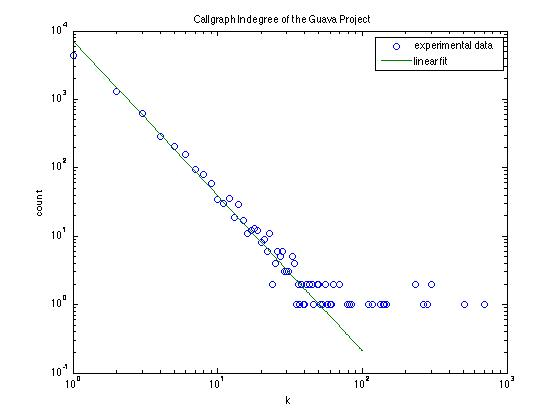
\includegraphics[width=1.2\textwidth]{dist.jpg}}
  \end{column}
\end{columns}
}

\section{Limitations} 
\frame{\frametitle{Limitations} 
\begin{itemize}
  \item Can't give a precise runtime analysis, only an approximation.
    \vspace{\baselineskip}
  \item Requires the assumption that the overall runtime is approximately
    monotone with respect to the complexity of the functions.
\end{itemize}
}

\section{Questions}
\begin{frame}[plain,c]
  \begin{center}{\huge Questions?}\end{center}
\end{frame}

\end{document}

